\subsection{Auswertung}
\subsubsection{Ermittlung der Anregungsenergie}
Für jeden aufgenommenen Datensatz wird die Anodenspannung gegen die Beschleunigungsspannung aufgetragen (siehe Abb. \ref{fig:159K4V}, \ref{fig:kennlinien1} und \ref{fig:kennlinien2}). Der Fehler für beide Spannungen wird auf $0,05$ V geschätzt, da die aufgenommenen Spannungen nur auf zwei Nachkommastellen genau abgespeichert werden. Für die quantitative Auswertung wird eine Regressionskurve
\begin{align*}
  U_\mathrm{A}(U_\mathrm{B})=U_0+\alpha U_\mathrm{B}+\sum_{K=1}^nA_k\exp \left(-\frac{(U_\mathrm{B}-\mu_k)^2}{2\sigma_k^2} \right)
\end{align*}
angepasst. Dabei steht $n$ jeweils für die Zahl der erkennbaren Spannungsmaxima. Die resultierenden Parameter sind in Tabelle \ref{tab:fh_parameter_1} und \ref{tab:fh_parameter_2} zu sehen. Nun wird der Abstand von aufeinanderfolgenden $\mu$ bestimmt (Tabelle \ref{tab:fh_dist}). Dieser Abstand entspricht dem mittleren Abstand von zwei Spannungsmaxima. Der Abstand zum fünften Maximum wird dabei nicht verwendet, da dieses nicht komplett zu erkennen ist. Berechnet man den varianzgewichteten Mittelwert erhält man 
\begin{align*}
  \Delta \mu=(4,89 \pm 0,01)\mathrm{\ V.}
\end{align*}
Der von uns betrachtete Übergang hat also die Energiedifferenz $(4,89 \pm 0,01)$ eV.
Laut \cite{praktikumsheft} entspricht dies genau dem Übergang $6^1S_0 \ \rightarrow \ 6^3P_1$ von Quecksilber.

\begin{figure}[!h]
  \centering
  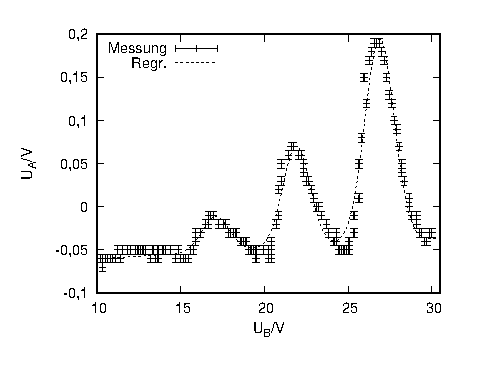
\includegraphics[width=0.55\textwidth]{data/fh/159K4V.eps}
  \caption{Anodenspannung bei $T=159^\circ$C und $U_\mathrm{G}=4$ V}
  \label{fig:159K4V}
\end{figure}

\newpage

\begin{figure}[!h]
  \centering
  \begin{subfigure}[h]{0.5\textwidth}
    \centering
    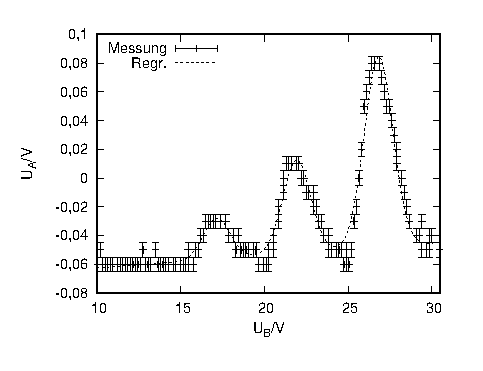
\includegraphics{data/fh/168K4V.eps}
    \subcaption{$T=168^\circ$C}
  \end{subfigure}%
  \begin{subfigure}[h]{0.5\textwidth}
    \centering
    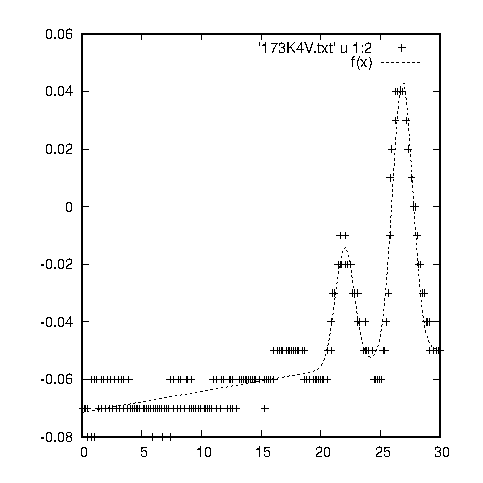
\includegraphics{data/fh/173K4V.eps}
    \subcaption{$T=173^\circ$C}
  \end{subfigure}
    \begin{subfigure}[h]{0.5\textwidth}
    \centering
    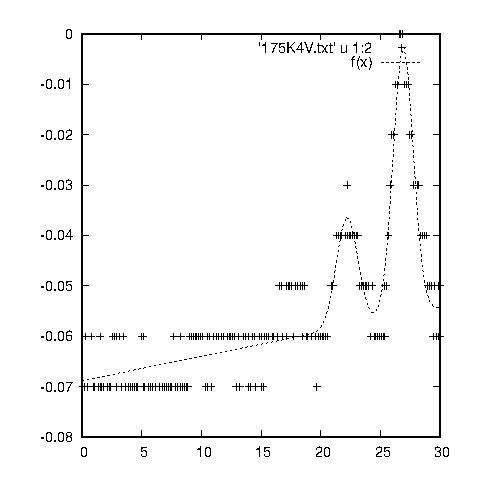
\includegraphics{data/fh/175K4V.eps}
    \subcaption{$T=175^\circ$C}
  \end{subfigure}%
  \begin{subfigure}[h]{0.5\textwidth}
    \centering
    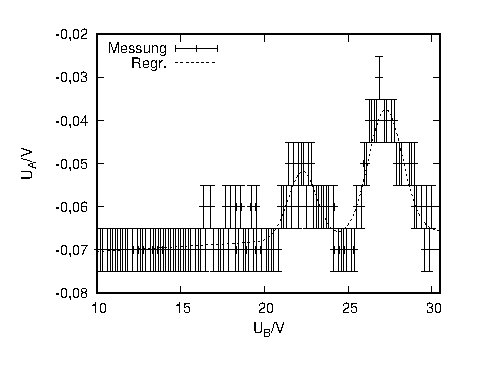
\includegraphics{data/fh/181K4V.eps}
    \subcaption{$T=181^\circ$C}
  \end{subfigure}
  \caption{Anodenspannung für weitere Temperaturen}
  \label{fig:kennlinien1}
\end{figure}

\newpage

\begin{figure}[!h]
  \centering
  \begin{subfigure}[h]{0.5\textwidth}
    \centering
    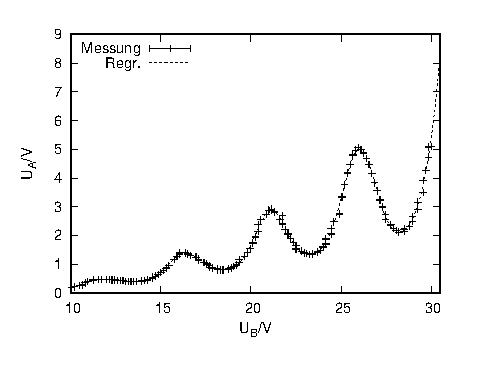
\includegraphics{data/fh/165K1V.eps}
    \subcaption{$U_\mathrm{G}=1$V}
  \end{subfigure}%
  \begin{subfigure}[h]{0.5\textwidth}
    \centering
    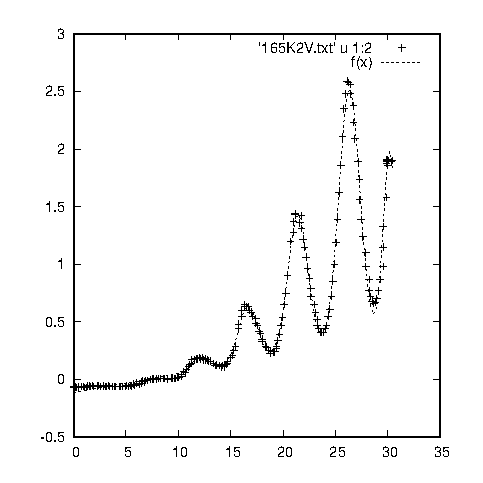
\includegraphics{data/fh/165K2V.eps}
    \subcaption{$U_\mathrm{G}=2$V}
  \end{subfigure}
    \begin{subfigure}[h]{0.5\textwidth}
    \centering
    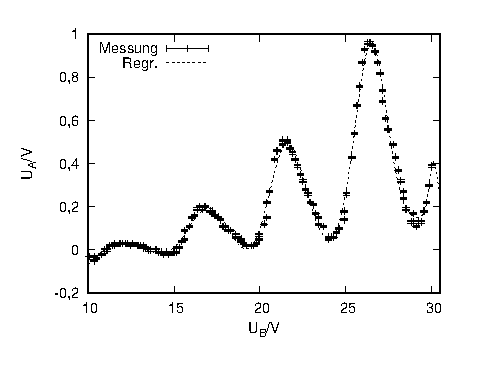
\includegraphics{data/fh/165K3V.eps}
    \subcaption{$U_\mathrm{G}=3$V}
  \end{subfigure}%
  \begin{subfigure}[h]{0.5\textwidth}
    \centering
    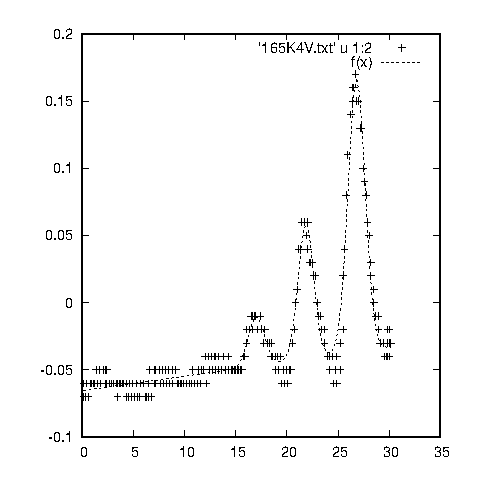
\includegraphics{data/fh/165K4V.eps}
    \subcaption{$U_\mathrm{G}=4$V}
  \end{subfigure}
  \caption{Anodenspannung für verschiedene Gegenspannungen bei $165^\circ$ C}
  \label{fig:kennlinien2}
\end{figure}

\newpage

\subsubsection{Dominanz eines Übergangs}
In Abbildung \ref{fig:wirkungsquerschnitt} ist der energieabhängige Wirkungsquerschnitt von Quecksilber für vier verschiedene Übergänge zu sehen. An der Abbildung kann erklärt werden, warum ein Übergang für den Versuch dominant ist. Übergang eins hat den maximalen Wirkungsquerschnitt bei einer leicht kleinerern Energie als Übergang zwei. Übergang zwei hat allerdings einen deutlich größeren maximalen Wirkungsquerschnitt, weshalb dieser hier dominant ist. Übergang drei und vier können ebenfalls vernachlässigt werden, da es sehr wahrscheinlich ist, dass die Elektronen Energie durch den Übergang zwei abgeben und somit keine Energien erreichen um die Übergänge drei und vier auszulösen.

\begin{figure}[h]
  \centering
  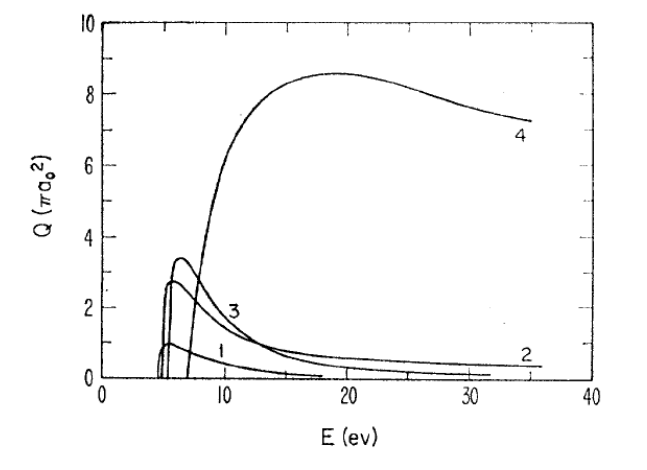
\includegraphics[width=0.6\textwidth]{data/fh/wirkungsquerschnitt.png}
  \caption{Totaler Wirkungsquerschnitt von Hg für Elektronenstoßanregung aus \cite{wirkungsquerschnitt}\\ 1: $6^1S_0\rightarrow 6^3P_0$, \   2: $6^1S_0\rightarrow 6^3P_1$, \   3: $6^1S_0\rightarrow 6^3P_2$, \   4: $6^1S_0\rightarrow 6^1P_1$}
  \label{fig:wirkungsquerschnitt}
\end{figure}

\subsubsection{Einfluss von Gegenspannung und Temperatur}
An den angepassten Regressionskurven ist zu erkennen, dass sich, wie erwartet, die Größen $\mu$ und $\sigma$ kaum mit Temperatur und Gegenspannung ändern. Die Elektronen weisen nach dem Gitter eine gewisse Geschwindigkeitsverteilung auf. Für kleine Erhöhungen der Gegenspannung wird deshalb eine lineare Abnahme der Anodenspannung erwartet. In Abbildung \ref{fig:abh} wurden die Amplituden von verschiedenen Maxima der Anodenspannung gegen die Gegenspannung aufgetragen. Wie erwartet zeigt sich näherungsweise eine lineare Abhängigkeit.

\begin{figure}[h]
  \centering
  \begin{subfigure}[h]{0.5\textwidth}
    \centering
    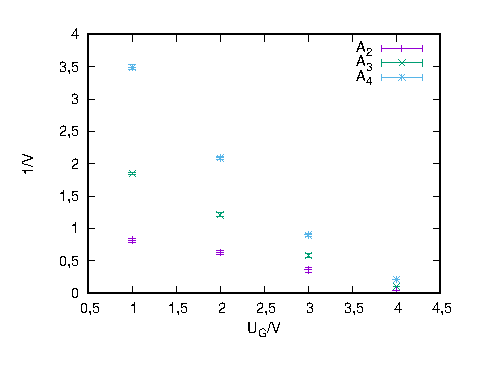
\includegraphics{data/fh/abh_u.eps}
  \end{subfigure}%
  \begin{subfigure}[h]{0.5\textwidth}
    \centering
    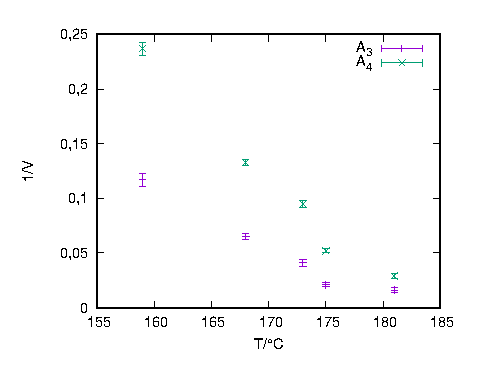
\includegraphics{data/fh/abh_t.eps}
  \end{subfigure}
  \caption{Abhängigkeit des Anodenstroms zur Gegenspannung und Temperatur}
  \label{fig:abh}
\end{figure}

Erhöht man den Druck in der Gasentladungsröhre ist es wahrscheinlicher, dass ein Elektron ein Atom zum Stoßen findet. Dadurch sollten die Maxima des Anodenstroms bei steigendem Druck (bzw. steigender Temperatur) sinken. Dieses Verhalten kann mit Abbildung \ref{fig:abh} auch bestätigt werden. Mit Abbildung \ref{fig:druck} lässt sich nachvollziehen, warum der Versuch praktisch auf ein kleines Temperaturintervall beschränkt ist. Für zu kleine Temperaturen geht der Druck schnell gegen null und die Elektronen stoßen kaum. Für zu große Temperaturen stoßen die Elektronen sehr oft (auch elastisch) und schaffen es nicht mehr, die Gegenspannung zu überwinden.

\newpage

\begin{figure}[!h]
  \centering
  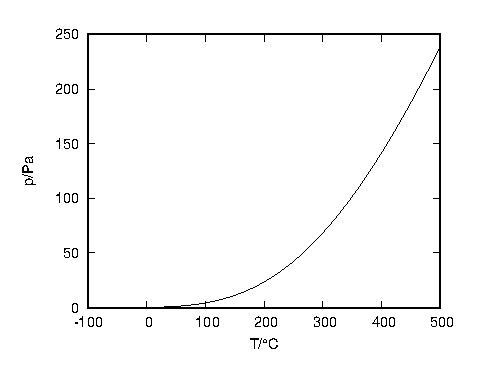
\includegraphics[width=0.7\textwidth]{data/fh/druck.eps}
  \caption{Dampfdruckkurve von Quecksilber, funktionaler Zusammenhang aus \cite{praktikumsheft}}
  \label{fig:druck}
\end{figure}
